
\begin{frame}{The Basic Source Coding Problem}
  \vspace{-1ex}
\STRUC{Basic Source Coding Problem}
\bit
\item Two equivalent formulations:
  \begin{center}\begin{minipage}{0.8\linewidth}
  \basblk{}
  \ALERT{\begin{center}
    Representing source data with highest fidelity possible\\
    within an available bit rate
  \end{center}}
  \easblk
  \end{minipage}\end{center}
\uncover<2->{and
  \begin{center}\begin{minipage}{0.8\linewidth}
  \basblk{}
  \ALERT{\begin{center}
    Representing source data using lowest bit rate possible\\
    while maintaining a specified reproduction quality
  \end{center}}
  \easblk
  \end{minipage}\end{center}}
\eit

  \bigskip
\uncover<3->{\STRUC{Source Codec}
  \bit
  \item Source \ALERT{codec}: System of en\ALERT{co}der and \ALERT{dec}oder
    \eit
    \vspace{-1ex}
\begin{center}
\fitbox{\linewidth}{0.1\textheight}{\relsize{-2}%
  \smallskip
  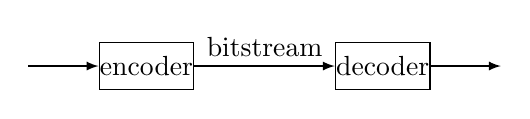
\begin{tikzpicture}
  [
    pstep/.style={
      draw=black,
      fill=white,
      line width=0.5pt,
      minimum width=1.2cm,
      minimum height=0.6cm,
      inner sep=0,
      align=center
    },
    nbox/.style={pstep,
      rectangle
    },
    narrow/.style={
      ->,
      >=latex,
      line width=0.5pt
    },
    step=.5cm
  ]
  \node[] (videoenc)   [nbox]    at (5,5) {encoder};
  \node[] (videodec)   [nbox]    at (8,5) {decoder};
  \draw[] [narrow] (3.5,5)  -- (videoenc);
  \draw[] [narrow] (videoenc) -- (videodec)  node [pos=0.5,anchor=south] {bitstream};
  \draw[] [narrow] (videodec) -- (9.5,5);
  \end{tikzpicture}}%
  \smallskip
\end{center}
}
\end{frame}
